\documentclass[aspectratio=169,13pt]{beamer}
\usepackage{FAU-beamer}
\usepackage[ngerman,english]{babel}
\usepackage{xcolor}
\usepackage{amsmath}
\usepackage{amsfonts}
\usepackage{amssymb}
\usepackage{etoolbox}
\usepackage{pgfplots}
\usepackage{tikz}
\usepackage{enumitem}
\usepackage{mathtools}
\usepackage{euler}
\usepackage{tikz-3dplot}
\usepackage{fontspec}
\usepackage{kbordermatrix}
\usepackage{pgfplots}
\pgfplotsset{width=14cm, height = 3cm, compat=1.8}
\usepackage[rm={lining,proportional},sf={lining,proportional},tt={lining,tabular,monowidth}]{cfr-lm}
\usepgfplotslibrary{patchplots}
\usetikzlibrary{patterns, positioning, arrows, fadings, shadows.blur, calc,intersections,fadings,backgrounds, decorations.markings,arrows.meta,bending}
\tikzfading[name=fade out, inner color=transparent!0, outer color=transparent!100]
\usepackage[
bibstyle=authoryear,
citestyle=authoryear,
maxcitenames=2,
maxbibnames=100,
backend=bibtex
]{biblatex}
\usepgfplotslibrary{external} 
\tikzexternalize
\hypersetup{
    unicode=true,
    pdfencoding=unicode,
    pdftoolbar=false,
    pdfmenubar=false,
    pdffitwindow=false,
    pdfstartview={FitH},
    pdftitle={Introduction to Persistent Homology},
    pdfauthor={Luciano Melodia},
    pdfsubject={Topological Data Analysis},
    pdfcreator={Luciano Melodia},
    pdfproducer={XeLaTeX},
    pdfnewwindow=false,
    colorlinks=false,
    linkcolor=FAURed,
    urlcolor=true
}
\newcommand\Fontvi{\fontsize{14}{14}\selectfont}
\definecolor{navy}{RGB}{2, 105, 164}
\newcommand\col{\bfseries}
\RequirePackage[oldstyle,scale=1]{sourcecodepro}
\RequirePackage{dsfont}
\setbeamertemplate{bibliography item}{\insertbiblabel}
\defbeamertemplate*{title page}{customized}[1][]
{
  \placelogofalse
  \usebeamerfont{title}\inserttitle\par
  \usebeamerfont{subtitle}\insertsubtitle\par
  \usebeamerfont{author}\insertauthor\par
}

\mode<presentation>{
    \AtBeginSection[]{
    	\begin{frame}
    	\vfill
    	\centering
    	\begin{beamercolorbox}[sep=8pt,center]{title}
    	\huge{\color{black}\insertsectionhead}\par%
    	\end{beamercolorbox}
    	\vfill
    	\end{frame}
    }
}

\tikzset{->-/.style={decoration={markings,mark=at position #1 with {\arrow[line width=0.7pt]{>}}},postaction={decorate}}}

\setbeamertemplate{frametitle}{\bfseries
\hspace{-0.75cm}\insertframetitle}
\setbeamertemplate{theorems}[numbered]
\theoremstyle{plain}
\newtheorem{proposition}{Proposition}
\def\maketitle{\ifbeamer@inframe\titlepage\else\frame{\titlepage}\fi}


\title{\textbf{Introduction to Persistent Homology}}
\author{Luciano Melodia}
\institute[Chair of Computer Science 6]{}

\begin{document}
\begin{frame}[plain,noframenumbering]
    \titlepage
\end{frame}

\placelogotrue

\begin{frame}
\frametitle{
Data manifolds
\par\hspace{-0.7cm}
\footnotesize{Underlying spaces}}
\centering
\tdplotsetmaincoords{75}{70}
\begin{tikzpicture}[tdplot_main_coords,scale=3.14]
\draw[name path=back] plot[variable=\x,samples=180,domain=90:270]
({1.2*cos(\x)},{sin(\x)},{1.6-0.4*cos(2*\x)});
\draw[name path=front] plot[variable=\x,samples=180,domain=-90:90]
({1.2*cos(\x)},{sin(\x)},{1.6-0.4*cos(2*\x)}); 
\coordinate (front1) at ({1.2*cos(-45)},{sin(-45)},{1.6-0.4*cos(-2*45)});
\coordinate (front2) at ({1.2*cos(45)},{sin(45)},{1.6-0.4*cos(2*45)});
\coordinate (front3) at ({1.2*cos(0)},{sin(0)},{1.6-0.4*cos(2*0)});
\draw[name path=top,opacity=0.3] plot[variable=\x,samples=180,domain=-90:90]
(0,{sin(\x)},{1.8-0.2*cos(2*\x)});
\coordinate (top1) at (0,{sin(0)},{1.8-0.2*cos(2*0)});
\path[name intersections={of=top and back, by={tb}}];
\draw[name path=top front,opacity=0.3] (front1)  to[out=-10,in=-150] (front2);
\draw[name path=top front,opacity=0.3] (front3)  to[out=100,in=-20] (top1)
to[out=160,in=20] (tb);
\fill[FAURed,opacity=0.5] plot[variable=\x,samples=180,domain=-90:90]
(0,{sin(\x)},{1.8-0.2*cos(2*\x)}) --
plot[variable=\x,samples=180,domain=90:-90]
({1.2*cos(\x)},{sin(\x)},{1.6-0.4*cos(2*\x)});

\fill[FAURed,opacity=0.3] plot[variable=\x,samples=180,domain=-90:90]
(0,{sin(\x)},{1.8-0.2*cos(2*\x)}) --
plot[variable=\x,samples=180,domain=90:270]
({1.2*cos(\x)},{sin(\x)},{1.6-0.4*cos(2*\x)});
\end{tikzpicture}
\\[0.5cm]
What if this \textbf{manifold} describes a set of points close to perfection?\\
How can we determine a suitable \textbf{topology} for a given set of points?
\end{frame}


\begin{frame}{Overview}
\Fontvi
\textbf{\color{FAURed}I}: \hspace{0.45cm} Motivation\\[0.2cm]
\textbf{\color{FAURed}II}: \hspace{0.3cm} Simplicial complexes\\[0.2cm]
\textbf{\color{FAURed}III}: \hspace{0.12cm} Filtrations\\[0.2cm]
\textbf{\color{FAURed}IV}: \hspace{0.1cm} Homology groups\\[0.2cm]
\textbf{\color{FAURed}V}: \hspace{0.25cm} Persistent homology\\[0.2cm]
\end{frame}

\section{Part I: \textbf{\color{FAURed}Motivation}}

\begin{frame}
\frametitle{
Data manifolds
\par\hspace{-0.7cm}
\footnotesize{The structure of data}}
\centering
\begin{tikzpicture}
    \tikzstyle{point}=[circle,thick,draw=FAURed,fill=FAURed,inner sep=0pt,minimum width=4pt,minimum height=4pt]
    \node (a)[point] at (0.4,0) {};
    \node (b)[point] at (1,1) {};
    \node (c)[point] at (2,1) {};
    \node (d)[point] at (2.6,0) {};
    \node (e)[point] at (2,-1) {};
    \node (f)[point] at (1,-1) {};
\end{tikzpicture}
\\[0.5cm]
There exists at least a \textbf{topological manifold} underlying the data.\\
A \textbf{dataset} is a set of points embedded in some $\mathbb{R}^n$.
\end{frame}

\begin{frame}
\frametitle{
Data manifolds
\par\hspace{-0.7cm}
\footnotesize{The structure of data}}
\centering
\begin{tikzpicture}
    \tikzstyle{point}=[circle,thick,draw=black,fill=black,inner sep=0pt,minimum width=4pt,minimum height=4pt]
    \fill[FAUSilver,opacity=0.2] (0.4,0) circle (0.25);
    \fill[FAUSilver,opacity=0.2] (1,1) circle (0.25);
    \fill[FAUSilver,opacity=0.2] (2,1) circle (0.25);
    \fill[FAUSilver,opacity=0.2] (2.6,0) circle (0.25);
    \fill[FAUSilver,opacity=0.2] (2,-1) circle (0.25);
    \fill[FAUSilver,opacity=0.2] (1,-1) circle (0.25);
    \node (a)[point] at (0.4,0) {};
    \node (b)[point] at (1,1) {};
    \node (c)[point] at (2,1) {};
    \node (d)[point] at (2.6,0) {};
    \node (e)[point] at (2,-1) {};
    \node (f)[point] at (1,-1) {};
\end{tikzpicture}
\\[0.5cm]
How can we make the \textbf{topological structure} of the underlying space visible?\\
We span a \textbf{simplicial complex} using closed balls starting with radius $r=0.25$.
\end{frame}

\begin{frame}
\frametitle{
Data manifolds
\par\hspace{-0.7cm}
\footnotesize{The structure of data}}
\centering
\begin{tikzpicture}
    \tikzstyle{point}=[circle,thick,draw=black,fill=black,inner sep=0pt,minimum width=4pt,minimum height=4pt]
    \fill[FAUSilver,opacity=0.2] (0.4,0) circle (0.5);
    \fill[FAUSilver,opacity=0.2] (1,1) circle (0.5);
    \fill[FAUSilver,opacity=0.2] (2,1) circle (0.5);
    \fill[FAUSilver,opacity=0.2] (2.6,0) circle (0.5);
    \fill[FAUSilver,opacity=0.2] (2,-1) circle (0.5);
    \fill[FAUSilver,opacity=0.2] (1,-1) circle (0.5);
    \node (a)[point] at (0.4,0) {};
    \node (b)[point] at (1,1) {};
    \node (c)[point] at (2,1) {};
    \node (d)[point] at (2.6,0) {};
    \node (e)[point] at (2,-1) {};
    \node (f)[point] at (1,-1) {};
    \draw (b.center) -- (c.center);
    \draw (e.center) -- (f.center);
\end{tikzpicture}
\\[0.5cm]
No additional \textbf{simplex} is created, thus we enlarge the radius.\\
This \textbf{simplicial complex} is spanned with an $r=0.5$.
\end{frame}

\begin{frame}
\frametitle{
Data manifolds
\par\hspace{-0.7cm}
\footnotesize{The structure of data}}
\centering
\begin{tikzpicture}
    \tikzstyle{point}=[circle,thick,draw=black,fill=black,inner sep=0pt,minimum width=4pt,minimum height=4pt]
    \fill[FAUSilver,opacity=0.2] (0.4,0) circle (0.85);
    \fill[FAUSilver,opacity=0.2] (1,1) circle (0.85);
    \fill[FAUSilver,opacity=0.2] (2,1) circle (0.85);
    \fill[FAUSilver,opacity=0.2] (2.6,0) circle (0.85);
    \fill[FAUSilver,opacity=0.2] (2,-1) circle (0.85);
    \fill[FAUSilver,opacity=0.2] (1,-1) circle (0.85);
    \node (a)[point] at (0.4,0) {};
    \node (b)[point] at (1,1) {};
    \node (c)[point] at (2,1) {};
    \node (d)[point] at (2.6,0) {};
    \node (e)[point] at (2,-1) {};
    \node (f)[point] at (1,-1) {};
    \draw (a.center) -- (b.center) -- (c.center) -- (d.center) -- (e.center) -- (f.center) -- cycle;
\end{tikzpicture}
\\[0.5cm]
Whenever two of the \textbf{closed balls} touch, an edge is created.\\
This \textbf{simplicial complex} is spanned with an $r=0.85$.\\
This simplicial complex is called $1$-skeleton or $K^{(1)}$, with $\dim \sigma \leq 1$.
\end{frame}


\begin{frame}
\frametitle{
Data manifolds
\par\hspace{-0.7cm}
\footnotesize{The structure of data}}
\centering
\begin{tikzpicture}
    \tikzstyle{point}=[circle,thick,draw=black,fill=black,inner sep=0pt,minimum width=4pt,minimum height=4pt]
    \fill[FAUSilver,opacity=0.2] (0.4,0) circle (1);
    \fill[FAUSilver,opacity=0.2] (1,1) circle (1);
    \fill[FAUSilver,opacity=0.2] (2,1) circle (1);
    \fill[FAUSilver,opacity=0.2] (2.6,0) circle (1);
    \fill[FAUSilver,opacity=0.2] (2,-1) circle (1);
    \fill[FAUSilver,opacity=0.2] (1,-1) circle (1);
    \node (a)[point] at (0.4,0) {};
    \node (b)[point] at (1,1) {};
    \node (c)[point] at (2,1) {};
    \node (d)[point] at (2.6,0) {};
    \node (e)[point] at (2,-1) {};
    \node (f)[point] at (1,-1) {};
    \filldraw[draw=black, fill=FAURed] (a.center) -- (c.center) -- (b.center) -- (a.center) -- cycle;
    \filldraw[draw=black, fill=FAURed] (b.center) -- (d.center) -- (c.center) -- (b.center) -- cycle;
    \filldraw[draw=black, fill=FAURed] (c.center) -- (e.center) -- (d.center) -- (c.center) -- cycle;
    \filldraw[draw=black, fill=FAURed] (d.center) -- (f.center) -- (e.center) -- (d.center) -- cycle;
    \filldraw[draw=black, fill=FAURed] (e.center) -- (a.center) -- (f.center) -- (e.center) -- cycle;
    \filldraw[draw=black, fill=FAURed] (f.center) -- (b.center) -- (a.center) -- (f.center) -- cycle;
    \draw (a.center) -- (b.center) -- (c.center) -- (d.center) -- (e.center) -- (f.center) -- cycle;
    \draw (d.center) -- (f.center);
    \draw (c.center) -- (e.center);
    \draw (b.center) -- (d.center);
    \draw (e.center) -- (a.center);
    \draw (a.center) -- (c.center);
    \node (a)[point] at (0.4,0) {};
    \node (b)[point] at (1,1) {};
    \node (c)[point] at (2,1) {};
    \node (d)[point] at (2.6,0) {};
    \node (e)[point] at (2,-1) {};
    \node (f)[point] at (1,-1) {};
\end{tikzpicture}
\\[0.5cm]
Whenever three or more of the \textbf{closed balls} touch, a \textbf{$2$-simplex} is created.\\
This \textbf{simplicial complex} is spanned with an $r=1.0$.
\end{frame}

\begin{frame}
\frametitle{
Data manifolds
\par\hspace{-0.7cm}
\footnotesize{The structure of data}}
\centering
\begin{tikzpicture}
    \tikzstyle{point}=[circle,thick,draw=black,fill=black,inner sep=0pt,minimum width=4pt,minimum height=4pt]
    \fill[FAUSilver,opacity=0.2] (0.4,0) circle (1.25);
    \fill[FAUSilver,opacity=0.2] (1,1) circle (1.25);
    \fill[FAUSilver,opacity=0.2] (2,1) circle (1.25);
    \fill[FAUSilver,opacity=0.2] (2.6,0) circle (1.25);
    \fill[FAUSilver,opacity=0.2] (2,-1) circle (1.25);
    \fill[FAUSilver,opacity=0.2] (1,-1) circle (1.25);
    \node (a)[point] at (0.4,0) {};
    \node (b)[point] at (1,1) {};
    \node (c)[point] at (2,1) {};
    \node (d)[point] at (2.6,0) {};
    \node (e)[point] at (2,-1) {};
    \node (f)[point] at (1,-1) {};
    \draw (a.center) -- (b.center) -- (c.center) -- (d.center) -- (e.center) -- (f.center) -- cycle;
    \filldraw[draw=black, fill=FAURed] (a.center) -- (c.center) -- (b.center) -- (a.center) -- cycle;
    \filldraw[draw=black, fill=FAURed] (a.center) -- (e.center) -- (b.center) -- (a.center) -- cycle;
    \filldraw[draw=black, fill=FAURed] (b.center) -- (e.center) -- (c.center) -- (b.center) -- cycle;
    \filldraw[draw=black, fill=FAURed] (c.center) -- (e.center) -- (d.center) -- (c.center) -- cycle;
    \draw (b.center) -- (d.center);
    \filldraw[draw=black, fill=FAURed] (d.center) -- (f.center) -- (e.center) -- (d.center) -- cycle;
    \filldraw[draw=black, fill=FAURed] (e.center) -- (a.center) -- (f.center) -- (e.center) -- cycle;
    \filldraw[draw=black, fill=FAURed] (f.center) -- (b.center) -- (a.center) -- (f.center) -- cycle;
    \draw (e.center) -- (a.center);
    \draw (a.center) -- (c.center);
    \draw (d.center) -- (f.center);
    \draw (c.center) -- (e.center);
    \draw (a.center) -- (d.center);
    \draw (b.center) -- (e.center);
    \draw (c.center) -- (f.center);
    \node (a)[point] at (0.4,0) {};
    \node (b)[point] at (1,1) {};
    \node (c)[point] at (2,1) {};
    \node (d)[point] at (2.6,0) {};
    \node (e)[point] at (2,-1) {};
    \node (f)[point] at (1,-1) {};
\end{tikzpicture}
\\[0.5cm]
When no more additional \textbf{simplices} appear, we have a \textbf{triangulation}.\\
This \textbf{triangulation} does not embed into $\mathbb{R}^2$, but into $\mathbb{R}^3$.
\end{frame}


\section{Part II: \textbf{\color{FAURed}Simplicial complexes}}
\begin{frame}
    \frametitle{
    Simplices\par\hspace{-0.7cm}
    \small{Building blocks}}
    \Fontvi
    Given a set $X = \{x_0, \cdots, x_k\} \subset \mathbb{R}^d$ of $k+1$ points that \textbf{do not lie on a hyperplane with dimension less than $d$}, the $k$-dimensional simplex $v$ spanned by $X$ is the \textbf{set of convex combinations}
    \begin{align}
      \sum_{i=0}^{k} \lambda_i x_i \quad \text{with} \quad \sum_{i=0}^{k} \lambda_i = 1 \quad \text{and} \quad \lambda_i \geq 0.
    \end{align}
\end{frame}

\begin{frame}
    \frametitle{
    Simplices\par\hspace{-0.7cm}
    \small{Examples}}
    \Fontvi
    \centering
    \begin{tikzpicture}
        \node[anchor=south west,inner sep=0] (image) at (2,0) {
        
\includegraphics[width=0.2cm]{0-simplex.pdf}};
        \node[anchor=south west,inner sep=0] (image) at (4,0) {
        
\includegraphics[width=2cm]{1-simplex.pdf}};
        \node[anchor=south west,inner sep=0] (image) at (8,0) {
        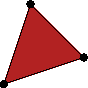
\includegraphics[width=2cm]{2-simplex.pdf}};
        \node[anchor=south west,inner sep=0] (image) at (12,0) {
        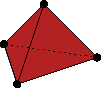
\includegraphics[width=2cm]{3-simplex.pdf}};
        \node[anchor=south west] at (1.82,0.13) {$a$};
        \node[anchor=south west] at (3.8,0.13) {$a$};
        \node[anchor=south west] at (5.63,0.13) {$b$};
        \node[anchor=south west] at (7.5,-0.17) {$a$};
        \node[anchor=south west] at (9.85,0.3) {$b$};
        \node[anchor=south west] at (8.1,1.65) {$c$};
        \node[anchor=south west] at (11.8,-0.17) {$a$};
        \node[anchor=south west] at (13.85,0.3) {$b$};
        \node[anchor=south west] at (12.35,1.45) {$c$};
        \node[anchor=south west] at (11.45,0.5) {$d$};
    \end{tikzpicture}
    \\[0.5cm]
    \begin{flushleft}
        $0$-simplex \hspace{0.7cm} $1$-simplex  \hspace{1.7cm} $2$-simplex \hspace{1.9cm} $3$-simplex\\
        \hspace{0.4cm} point \hspace{1.2cm} segment \hspace{2cm} triangle \hspace{1.9cm} tetrahedron\\[0.5cm]
        \small{The coefficients $\lambda_i$ are chosen from the \textbf{vectorspace} $\mathbb{Z}_2 := \mathbb{Z}/2\mathbb{Z}$, such that we can \textbf{neglect the orientation} of the simplices. This is done for illustrative purposes, but can also be used for highly efficient computations.}
    \end{flushleft}
\end{frame}


\begin{frame}
    \frametitle{
    Abstract simplicial complexes\par\hspace{-0.7cm}
    \small{Definition}}
    \Fontvi
    Let $V$ be a finite set of vertices $\{v_1, \cdots, v_n\}$. Let $K$ be a set of subsets of $V$, such that all subsets of elements from $K$ also belong to $K$. Then we call the elements of $K$ \textbf{faces} and $K$ an \textbf{abstract simplicial complex}. \\[0.5cm]

    \small{The dimension of $K$ is the maximum dimension of any of its simplices. The underlying space is denoted by $\vert K \vert$. It is the union of its simplices together with the topology inherited from $\mathbb{R}^d$, with $d$ being the dimension of $K$.}
\end{frame}

\begin{frame}
    \frametitle{
    Abstract simplicial complexes\par\hspace{-0.7cm}
    \small{Example}}
    \Fontvi
    \centering
    \begin{tikzpicture}
        \tikzstyle{point}=[circle,thick,draw=black,fill=black,inner sep=0pt,minimum width=4pt,minimum height=4pt]
        \node[label=left:$v_1$, point] (a) at (0.4,0) {};
        \node[label=$v_2$, point] (b) at (1,1.4) {};
        \node[label=$v_3$, point] (c) at (3,0.4) {};
        \node[label=$v_4$, point] (d) at (5,0.8) {};
        \node[label=left:$v_5$, point] (e) at (1.8,-1.2) {};
        \node[label=left:$v_6$, point] (f) at (4,-1) {};

        \begin{scope}[on background layer]
            \filldraw[draw=black, fill=FAURed] (a.center) -- (b.center) -- (c.center) -- (a.center) -- cycle;
            \filldraw[draw=black, fill=FAURed] (a.center) -- (c.center) -- (e.center) -- (a.center) -- cycle;
            \filldraw[draw=black, fill=FAURed] (c.center) -- (d.center) -- (f.center) -- (c.center) -- cycle;
        \end{scope}
    \end{tikzpicture}
    \begin{align*}
    V = \; &\{v_1, v_2, v_3, v_4, v_5, v_6\}.\\
    K = \; &\{\{v_1\}, \cdots, \{v_6\}, \{\{v_1\},\{v_2\}\}, \cdots, \{\{v_4\},\{v_6\}\},\\
    &\{\{v_1\},\{v_2\},\{v_3\}\}, \cdots, \{\{v_3\},\{v_4\},\{v_6\}\}\}.
    \end{align*}
\end{frame}

\begin{frame}
    \frametitle{
    Geometric simplicial complexes\par\hspace{-0.7cm}
    \small{The geometric realization theorem}}
    \Fontvi
    \centering
    An \textbf{\color{FAURed}abstract simplicial complex} of dimension $d$\\ has a \textbf{geometric realization} in $\mathbb{R}^{2d+1}$.\\[0.5cm]
\end{frame}

\begin{frame}
    \frametitle{
    Geometric simplicial complexes\par\hspace{-0.7cm}
    \small{Proof of the geometric realization theorem}}
    \Fontvi
    Let $f: K^{(0)} \rightarrow \mathbb{R}^{2d+1}$ be injective, whose image is a \textbf{set of points in general position} ($2d + 2$ or fewer points are affinely independent).\\
    Let $\sigma$ and $\sigma_0$ be simplices in $K$ with $k = \dim \sigma$ and $k_0 = \dim \sigma_0$. \\
    Their union has size 
    \begin{align}
    \text{card} \; (\sigma \cup \sigma_0) &= \text{card} \;  \sigma + \text{card} \;  \sigma_0 - \text{card} \; (\sigma \cap \sigma_0) 
    \\ &\leq k + k_0 + 2 \leq 2d + 2.
    \end{align}
\end{frame}

\begin{frame}
    \frametitle{
    Geometric simplicial complexes\par\hspace{-0.7cm}
    \small{Proof of the geometric realization theorem}}
    \Fontvi
    The points in $\sigma \cup \sigma_0$ are affinely independent.\\
    $\implies$ Every \textbf{convex combination $x$ of points} in $\sigma \cup \sigma_0$ is unique.\\[0.2cm]
    Hence $x \in \tau = \text{conv} \; f(\sigma)$ as well $ x \in \tau_0 = \text{conv} \; f(\sigma_0)$, \\iff $x$ is a convex combination of $\sigma \cap \sigma_0$. \\
    $\implies$ The intersection of $\tau$ and $\tau_0$ is either empty or within $f(\sigma \cap \sigma_0)$.
\end{frame}

\begin{frame}
    \frametitle{
    Geometric simplicial complexes\par\hspace{-0.7cm}
    \small{Simplicial maps}}
    \Fontvi
    A \textbf{vertex map} is a function $\varphi: K^{(0)} \rightarrow L^{(0)}$ with the property that the vertices of every simplex in $K$ map to vertices of a simplex in $L$. Then $\varphi$ can be extended to a continuous map $f: \vert K \vert \rightarrow \vert L \vert$ defined by
    \begin{align}
        f(x) = \sum_{i=0}^{n} \lambda_i(x) \varphi(v_i).
    \end{align}
    This map is the \textbf{\color{FAURed}simplicial map} induced by $\varphi$.
\end{frame}

\section{Part III: \textbf{\color{FAURed}Filtrations}}

\begin{frame}
    \frametitle{
    Filtered (simplicial) complexes\par\hspace{-0.7cm}
    \small{Brief motivation}}
    \Fontvi
    We believe that different data comes from different \textbf{topological spaces}. How can we distinguish these using the data?\\[0.5cm]
    \emph{We don't want to distinguish data only by their \textbf{holes} of their \textbf{triangulation}, therefore we introduce a \textbf{magnifying glass} which allows us to capture the \textbf{structure of a topological space} in different granularity.}
\end{frame}

\begin{frame}
    \frametitle{
    Filtered (simplicial) complexes\par\hspace{-0.7cm}
    \small{Definition}}
    \Fontvi
    A \textbf{filtration} is a nested sequence of complexes $K_i$, which induce an ordering of the sublevel complexes. These complexes, together with the inclusion $K_i \hookrightarrow K_j$ for $0 \leq i \leq j \leq n$ is called a filtration and denoted by $\mathbb{K}$:
    \begin{align*}
        \mathbb{K}: \quad \emptyset = K_0 \subseteq K_1 \subseteq \cdots \subseteq K_n = K.
    \end{align}
    \small{The inclusion on the filtration induces a homomorphism of groups $f^{i,j}_k: H_k(K_i) \rightarrow H_k(K_j)$, in this case $H_k$ are the $k$-th homology groups.}
\end{frame}

\begin{frame}
    \frametitle{
    Filtered (simplicial) complexes\par\hspace{-0.7cm}
    \small{Example}}
    \Fontvi
    {\centering
    \begin{tikzpicture}
        \node[anchor=south west,inner sep=0] (image) at (2,0) {
        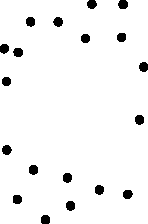
\includegraphics[width=2cm]{filtration-0.pdf}};
        \node[anchor=south west,inner sep=0] (image) at (5.5,0) {
        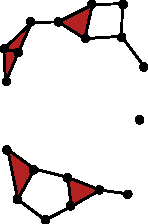
\includegraphics[width=2cm]{filtration-1.pdf}};
        \node[anchor=south west,inner sep=0] (image) at (9,0) {
        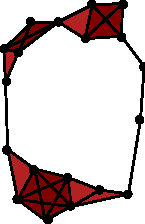
\includegraphics[width=2cm]{filtration-2.pdf}};
        \node[anchor=south west,inner sep=0] (image) at (12.5,0) {
        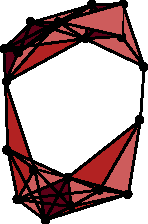
\includegraphics[width=2cm]{filtration-3.pdf}};
        \node[anchor=south west] at (4.3,1.1) {$\xhookrightarrow[]{\imath}$};
        \node[anchor=south west] at (7.8,1.1) {$\xhookrightarrow[]{\imath}$};
        \node[anchor=south west] at (11.3,1.1) {$\xhookrightarrow[]{\imath}$};
    \end{tikzpicture}}\\[0.5cm]
    \small{Vastly used complexes to create a filtration on a point set $X$ are:\\[0.2cm]
    \v{C}ech complex: \hspace{1.35cm} $(x_0, x_1, \cdots, x_k) \in \text{\v{C}ech}_r(X) \iff \bigcap_{i=0}^{k} B_{r}(x_i) \neq \emptyset$.\\
    Vietoris-Rips complex: \hspace{0.2cm} $(x_0, x_1, \cdots, x_k) \in \text{Rips}_{r}(X) \iff \vert\vert x_i - x_j || \leq r$.}
\end{frame}

\section{Part IV: \textbf{\color{FAURed}Homology groups}}

\begin{frame}
    \frametitle{
    Groups\par\hspace{-0.7cm}
    \small{Recall}}
    \Fontvi
    A \textbf{set} $G$ together with a map $+: G\times G \rightarrow G$, $(x,y) \mapsto x + y$ and an element $e = e_G$ are called \textbf{group}, iff

    \begin{enumerate}
        \item[{\color{FAURed} 1}.] $(xy)z = x(yz)$ for all $x,y,z \in G$,
        \item[{\color{FAURed} 2}.] $xe = ex = x$ for all $x \in G$,
        \item[{\color{FAURed} 3}.] for all $x \in G$ there exists $x^{-1} \in G$ such that $xx^{-1} = x^{-1}x = e$.
    \end{enumerate}\\[0.5cm]

    \small{If the group is abelian, which means commutative in every element under the operation, one denotes the group operation as $+$.}
\end{frame}

\begin{frame}
    \frametitle{
    Homomorphisms of groups\par\hspace{-0.7cm}
    \small{Recall}}
    \Fontvi
    A \textbf{homomorphism of groups} is a map $\varphi: G \rightarrow H$, with $G,H$ being groups, such that
    \begin{itemize}
        \item $\varphi(e_G) = e_H$,
        \item $\varphi(g_1 \star g_2) = \varphi(g_1) \circ \varphi(g_2)$.
    \end{itemize}
\end{frame}

\begin{frame}
    \frametitle{
    Chain groups\par\hspace{-0.7cm}
    \small{Definition}}
    \Fontvi
    The \textbf{\color{FAURed} $k$th chain group} of a \textbf{simplicial complex $K$} is $(C_k(K),+)$, the \textbf{free commutative group} on the (oriented) $k$-simplices. \\[0.5cm]
    An element of $C_k(K)$ is called $k$-chain, $\sum_{i} \lambda_i \sigma_i, \lambda_i \in \mathbb{Z}_2, \sigma_i \in K$.
\end{frame}

\begin{frame}
    \frametitle{
    Boundary homomorphism\par\hspace{-0.7cm}
    \small{Definition}}
    \Fontvi
    Let $K$ be a simplicial complex and $\sigma \in K$, $\sigma = [v_0,v_1,\cdots,v_k]$. The \textbf{\color{FAURed} boundary homomorphism} $\partial_k: C_k(K) \rightarrow C_{k-1}(K)$ is
    \begin{align}
        \partial_k \sigma = \sum_{i} (-1)^i [v_0, v_1,\cdots,\hat{v}_i,\cdots,v_n].
    \end{align}
\end{frame}

\begin{frame}
    \frametitle{
    Boundary homomorphism\par\hspace{-0.7cm}
    \small{Fundamental lemma}}
    \textbf{The composition $\partial_{k-1} \circ \partial _k$ is zero.}\\
    We have
    \begin{align}
        \partial_k(\sigma) = \sum_{i} (-1)^i \sigma \vert[v_0, \cdots, \hat{v}_i, \cdots, v_k],
    \end{align}
    and hence 
    \begin{align}
    \partial_{k-1}\partial_k(\sigma) = & \; \sum_{j<i} (-1)^i (-1)^j \sigma \vert[v_0, \cdots, \hat{v}_i, \cdots,\hat{v}_j, \cdots, v_k]\\
    &+ \sum_{j>i} (-1)^i (-1)^{j-1} \sigma \vert[v_0, \cdots, \hat{v}_i, \cdots,\hat{v}_j, \cdots, v_k].
    \end{align}
    The latter two summations cancel, as the second sum becomes the negative of the first after switching $i$ and $j$.
\end{frame}

\begin{frame}
    \frametitle{
    Cycle group\par\hspace{-0.7}}
    \Fontvi
    The \textbf{\color{FAURed}$k$th cycle group $Z_k$} is defined as
    \begin{align}
        Z_k &= \ker \partial_k\\
            &= \{c \in C_k \; | \; \partial_k c = 0\}.
    \end{align}
    An element of this group is called \textbf{$k$-cycle}.
\end{frame}

\begin{frame}
    \frametitle{
    Boundary group\par\hspace{-0.7}}
    \Fontvi
    The \textbf{\color{FAURed}$k$th boundary group $B_k$} is defined as
    \begin{align}
        B_k &= \text{im}\; \partial_{k+1}\\
            &= \{c \in C_k \; | \; \exists d \in C_{k+1}: c = \partial_{k+1} d\}.
    \end{align}
    An element of this group is called \textbf{$k$-boundary}.
\end{frame}


\begin{frame}
    \frametitle{
    Normal subgroup relation\par\hspace{-0.7cm}
    \small{Following Edelsbrunner, Zomorodian and many more}}
    \Fontvi
    \centering
    \begin{tikzpicture}
        \node[anchor=south west,inner sep=0] (image) at (2,0) {
        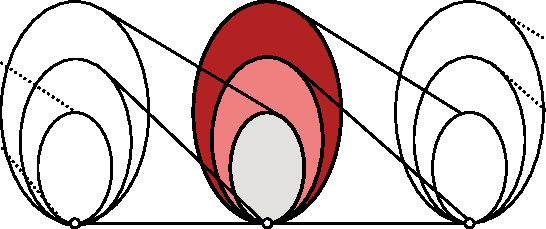
\includegraphics[width=0.7\textwidth]{groups.pdf}};
        \node[anchor=south west] at (3.05,-0.53) {$0$};
        \node[anchor=south west] at (6.5,-0.55) {$0$};
        \node[anchor=south west] at (10.14,-0.55) {$0$};
        \node[anchor=south west] at (2.7,3.2) {$C_{k+1}$};
        \node[anchor=south west] at (2.7,2.1) {$Z_{k+1}$};
        \node[anchor=south west] at (2.7,0.8) {$B_{k+1}$};
        \node[anchor=south west] at (6.4,3.2) {$C_k$};
        \node[anchor=south west] at (6.4,2.1) {$Z_k$};
        \node[anchor=south west] at (6.4,0.8) {$B_k$};
        \node[anchor=south west] at (9.8,3.2) {$C_{k-1}$};
        \node[anchor=south west] at (9.8,2.1) {$Z_{k-1}$};
        \node[anchor=south west] at (9.8,0.8) {$B_{k-1}$};
        \node[anchor=south west] at (8.2,3.2) {$\partial_{k}$};
        \node[anchor=south west] at (4.5,3.3) {$\partial_{k+1}$};
    \end{tikzpicture}\\
    \begin{flushleft}
    \small{A subgroup $B$ of a group $Z$ is normal with respect to $Z$, iff $zbz^{-1} \in B$. Thus, if it is invariant under conjugation. Normal subgroups are important. Only they can construct quotient groups.}
    \end{flushright}
\end{frame}

\begin{frame}
    \frametitle{
    Chain complex\par\hspace{-0.7cm}}
    \Fontvi
    \centering
    \begin{align}
      0 \xrightarrow[]{\partial_{k+1}} C_k \xrightarrow[]{\partial_{k}} C_{k-1} \xrightarrow[]{\partial_{k-1}} \cdots \xrightarrow[]{\partial_{2}} C_{1} \xrightarrow[]{\partial_{1}} 0
    \end{align}
\end{frame}

\begin{frame}
    \frametitle{
    Homology groups\par\hspace{-0.7cm}
    \small{Definition}}
    \Fontvi
    The $k$th \textbf{\color{FAURed}homology group} of a simplicial complex is defined as
    \begin{align}
      H_k(K) = \ker \partial_k C_k(K) / \text{im}\; \partial_{k+1} C_{k+1}(X).
    \end{align}
    Intuitively, the kernel of the boundary homomorphism of the $k$th chain group gives all $k$-cycles, thus the cycle group, from which we quotient out all elements of the $k$th boundary group, i.e. $H_k(K) = Z_k(K) / B_k(K)$.\\[0.5cm]

    \small{Technical details: Both subgroups, the cycle and boundary group, are normal because our chain groups are abelian.}
\end{frame}

\begin{frame}
    \frametitle{
    Homology groups\par\hspace{-0.7cm}
    \small{Example}}
    \setlength{\fboxsep}{0pt}
    \setlength{\fboxrule}{0pt}
    \fbox{
    \begin{minipage}{0.3\linewidth}
        \begin{tikzpicture}[bullet/.style={circle,fill,inner
        sep=1.5pt},>=latex, scale=0.5]
                \draw [black,line width=1pt,->-/.list={1/6,1/2,5/6}] 
                (210:3) node[bullet={below left:a}, label=left:$v_1$] (a) {}
                -- node[above left] {$e_1$} (90:3) node[bullet={above:b}, label=$v_2$] (b) {}
                -- node[above right] {$e_2$} (-30:3) node[bullet={below right:c}, label=right:$v_3$] (c) {}
                -- cycle;
                \draw [black,line width=1pt,->-/.list={2/6,5/6}] 
                (a) 
                -- node[below] {$e_5$} (-90:3) node[bullet={below right:c}, label=below:$v_4$] (d) {}
                -- node[below] {$e_4$} (c)
                -- cycle;
                \draw[line width=1pt,-{Latex[bend]}] (240:0.5) arc(240:-60:0.5);
            \begin{scope}[on background layer]
            \filldraw[draw=black, fill=FAURed] (a.center) -- (b.center) -- (c.center) -- node[below] {$e_3$} (a.center) -- cycle;
            \end{scope}
        \end{tikzpicture}
    \end{minipage}}%
    \fbox{%
    \begin{minipage}{0.7\linewidth}
        What we want to compute:
        \begin{align*}
        H_0(K)  &= \ker(\partial_0(C_0(K)))/ \text{im}\;(\partial_1(C_1(K)))\\
        &= C_0(K) / \text{im}(\partial_1(C_1(K)))
        \end{align*}

        Applying the boundary operator:
        \begin{align*}
        & \partial_1(c \in C_1(K)) = \partial_1(\lambda_1 e_1 + \lambda_2 e_2 + \lambda_3 e_3 + \lambda_4 e_4 + \lambda_5 e_5) \\
        = & \;\lambda_1(\partial_1(e_1)) + \lambda_2(\partial_1(e_2)) + \lambda_3(\partial_1(e_3)) \\
        &+ \lambda_4(\partial_1(e_4)) + \lambda_5(\partial_1(e_5))\\
        = &\;\lambda_1(v_2-v_1) + \lambda_2(v_3-v_2) + \lambda_3(v_1-v_3) \\
        &+ \lambda_4(v_3-v_4) + \lambda_5(v_4-v_1)\\
        \end{align*}
    \end{minipage}}
\end{frame}

\begin{frame}
    \frametitle{
    Homology groups\par\hspace{-0.7cm}
    \small{Example}}
    \setlength{\fboxsep}{0pt}
    \setlength{\fboxrule}{0pt}
    \fbox{
    \begin{minipage}{0.3\linewidth}
        \begin{tikzpicture}[bullet/.style={circle,fill,inner
        sep=1.5pt},>=latex, scale=0.5]
                \draw [black,line width=1pt,->-/.list={1/6,1/2,5/6}] 
                (210:3) node[bullet={below left:a}, label=left:$v_1$] (a) {}
                -- node[above left] {$e_1$} (90:3) node[bullet={above:b}, label=$v_2$] (b) {}
                -- node[above right] {$e_2$} (-30:3) node[bullet={below right:c}, label=right:$v_3$] (c) {}
                -- cycle;
                \draw [black,line width=1pt,->-/.list={2/6,5/6}] 
                (a) 
                -- node[below] {$e_5$} (-90:3) node[bullet={below right:c}, label=below:$v_4$] (d) {}
                -- node[below] {$e_4$} (c)
                -- cycle;
                \draw[line width=1pt,-{Latex[bend]}] (240:0.5) arc(240:-60:0.5);
            \begin{scope}[on background layer]
            \filldraw[draw=black, fill=FAURed] (a.center) -- (b.center) -- (c.center) -- node[below] {$e_3$} (a.center) -- cycle;
            \end{scope}
        \end{tikzpicture}
    \end{minipage}}%
    \fbox{%
    \begin{minipage}{0.7\linewidth}
        What we have computed:
        \begin{align*}
        & \; \partial_1(c \in C_1(K)) = \lambda_1(v_2-v_1) + \lambda_2(v_3-v_2) + \lambda_3(v_1-v_3) \\
        &+ \lambda_4(v_3-v_4) + \lambda_5(v_4-v_1)\\
        \end{align*}
        We bring this into matrix form:
        \renewcommand{\kbldelim}{(}% Left delimiter
        \renewcommand{\kbrdelim}{)}% Right delimiter
        \[
          M_{\partial_1(c)} = \kbordermatrix{
            & v_1 & v_2 & v_3 & v_4 & v_5 \\
            v_1 & -1 & 0 & 1 & 0 & -1 \\
            v_2 & 1 & -1 & 0 & 0 & 0 \\
            v_3 & 0 & 1 & -1 & 1 & 0 \\
            v_4 & 0 & 0 & 0 & -1 & 1 \\
            v_5 & 0 & 0 & 0 & 0 & 0
          }
        \]
    \end{minipage}}
\end{frame}

\begin{frame}
    \frametitle{
    Homology groups\par\hspace{-0.7cm}
    \small{Example}}
    \setlength{\fboxsep}{0pt}
    \setlength{\fboxrule}{0pt}
    \fbox{
    \begin{minipage}{0.3\linewidth}
        \begin{tikzpicture}[bullet/.style={circle,fill,inner
        sep=1.5pt},>=latex, scale=0.5]
                \draw [black,line width=1pt,->-/.list={1/6,1/2,5/6}] 
                (210:3) node[bullet={below left:a}, label=left:$v_1$] (a) {}
                -- node[above left] {$e_1$} (90:3) node[bullet={above:b}, label=$v_2$] (b) {}
                -- node[above right] {$e_2$} (-30:3) node[bullet={below right:c}, label=right:$v_3$] (c) {}
                -- cycle;
                \draw [black,line width=1pt,->-/.list={2/6,5/6}] 
                (a) 
                -- node[below] {$e_5$} (-90:3) node[bullet={below right:c}, label=below:$v_4$] (d) {}
                -- node[below] {$e_4$} (c)
                -- cycle;
                \draw[line width=1pt,-{Latex[bend]}] (240:0.5) arc(240:-60:0.5);
            \begin{scope}[on background layer]
            \filldraw[draw=black, fill=FAURed] (a.center) -- (b.center) -- (c.center) -- node[below] {$e_3$} (a.center) -- cycle;
            \end{scope}
        \end{tikzpicture}
    \end{minipage}}%
    \fbox{%
    \begin{minipage}{0.7\linewidth}
        What we have computed:\\[0.2cm]
        $M_{\partial_1(c)} = 
        \begin{pmatrix}
            -1 & 0 & 1 & 0 & -1\\
            1 & -1 & 0 & 0 & 0\\
            0 & 1 & -1 & 1 & 0\\
            0 & 0 & 0 & -1 & 1\\
            0 & 0 & 0 & 0 & 0\\
        \end{pmatrix}$\\[0.5cm]
        We conclude that: \\[0.2cm]
        $C_1(K) \simeq \mathbb{Z}^5$.\\
        What about $M_{\partial_1(c)}$?
    \end{minipage}}
\end{frame}

\begin{frame}
    \frametitle{
    Homology groups\par\hspace{-0.7cm}
    \small{Example}}
    \setlength{\fboxsep}{0pt}
    \setlength{\fboxrule}{0pt}
    \fbox{
    \begin{minipage}{0.3\linewidth}
        \begin{tikzpicture}[bullet/.style={circle,fill,inner
        sep=1.5pt},>=latex, scale=0.5]
                \draw [black,line width=1pt,->-/.list={1/6,1/2,5/6}] 
                (210:3) node[bullet={below left:a}, label=left:$v_1$] (a) {}
                -- node[above left] {$e_1$} (90:3) node[bullet={above:b}, label=$v_2$] (b) {}
                -- node[above right] {$e_2$} (-30:3) node[bullet={below right:c}, label=right:$v_3$] (c) {}
                -- cycle;
                \draw [black,line width=1pt,->-/.list={2/6,5/6}] 
                (a) 
                -- node[below] {$e_5$} (-90:3) node[bullet={below right:c}, label=below:$v_4$] (d) {}
                -- node[below] {$e_4$} (c)
                -- cycle;
                \draw[line width=1pt,-{Latex[bend]}] (240:0.5) arc(240:-60:0.5);
            \begin{scope}[on background layer]
            \filldraw[draw=black, fill=FAURed] (a.center) -- (b.center) -- (c.center) -- node[below] {$e_3$} (a.center) -- cycle;
            \end{scope}
        \end{tikzpicture}
    \end{minipage}}%
    \fbox{%
    \begin{minipage}{0.7\linewidth}
        After some Gaussian elimination:\\[0.2cm]
        $M_{\partial_1(c)} = 
        \begin{pmatrix}
            1 & 0 & -1 & 0 & 1\\
            0 & 1 & -1 & 0 & 1\\
            0 & 0 & 0 & 1 & -1\\
            0 & 0 & 0 & 0 & 0\\
            0 & 0 & 0 & 0 & 0\\
        \end{pmatrix}$\\[0.5cm]
        Thus $\text{rank}(M_{\partial_1(c)}) = 3$ and $M_{\partial_1(c)} \simeq \mathbb{Z}^3$.\\
        Therefore 
        \begin{align}
        H_0(K) &= C_0(K) / B_0(K) \simeq \mathbb{Z}^4 / M_{\partial_1(c)} \simeq \mathbb{Z}^4 / \mathbb{Z}^3  \simeq \mathbb{Z}.
        \end{align}
    \end{minipage}}
\end{frame}

\begin{frame}
    \frametitle{
    Betti numbers\par\hspace{-0.7}}
    \Fontvi
    The $k$th \textbf{Betti} number $\beta_k$ is the rank of the $k$th homology group $H_k(K)$ of the topological space $K$.\\[0.5cm]
    \small{We'll track the betti numbers to track the amount of holes along the filtration. Other properties of the vector space could also be helpful.}
\end{frame}


\section{Part V: \textbf{\color{FAURed}Persistent homology}}
\begin{frame}
    \frametitle{
    What is persistence?\par\hspace{-0.7}}
    \centering
    \begin{tikzpicture}
        \tikzstyle{point}=[circle,thick,draw=black,fill=black,inner sep=0pt,minimum width=4pt,minimum height=4pt]
        \fill[FAUSilver,opacity=0.2] (1.2,1) circle (0.6);
        \fill[FAUSilver,opacity=0.2] (2.2,1.1) circle (0.6);
        \fill[FAUSilver,opacity=0.2] (2,0) circle (0.6);
        \fill[FAUSilver,opacity=0.2] (1,0) circle (0.6);
        \node (f1)[point, opacity=0] at (2.5,1.7) {};
        \node (f2)[point, opacity=0] at (2.5,0.5) {};
        \node (f3)[point, opacity=0] at (2.3,1.7) {};
        \node (f4)[point, opacity=0] at (2.7,1.7) {};
        \node (f5)[point, opacity=0] at (2.3,0.5) {};
        \node (f6)[point, opacity=0] at (2.7,0.5) {};
        \node[anchor=south west] at (2.4,0.7) {$d_1$};
        \draw (f1.center) -- (f2.center);
        \draw (f3.center) -- (f4.center);
        \draw (f5.center) -- (f6.center);
        \node (a)[point] at (1.2,1) {};
        \node (b)[point] at (2.2,1.1) {};
        \node (c)[point] at (2,0) {};
        \node (d)[point] at (1,0) {};
        \draw (a.center) -- (b.center) -- (c.center) -- (d.center) -- cycle;
    \end{tikzpicture}\hspace{2cm}
    \begin{tikzpicture}
        \tikzstyle{point}=[circle,thick,draw=black,fill=black,inner sep=0pt,minimum width=4pt,minimum height=4pt]
        \node (a)[point] at (1.2,1) {};
        \node (b)[point] at (2.2,1.1) {};
        \node (c)[point] at (2,0) {};
        \node (d)[point] at (1,0) {};
        \node (p1)[point, opacity=0] at (2.5,1.8) {};
        \node (p2)[point, opacity=0] at (2.5,0.4) {};
        \node (p3)[point, opacity=0] at (2.3,1.8) {};
        \node (p4)[point, opacity=0] at (2.7,1.8) {};
        \node (p5)[point, opacity=0] at (2.3,0.4) {};
        \node (p6)[point, opacity=0] at (2.7,0.4) {};
        \node[anchor=south west] at (2.4,0.7) {$d_2$};
        \draw (a.center) -- (c.center);
        \draw (p1.center) -- (p2.center);
        \draw (p3.center) -- (p4.center);
        \draw (p5.center) -- (p6.center);
        \draw (a.center) -- (b.center) -- (c.center) -- (d.center) -- cycle;
        \begin{scope}[on background layer]
            \fill[FAUSilver,opacity=0.2] (1.2,1) circle (0.7);
            \fill[FAUSilver,opacity=0.2] (2.2,1.1) circle (0.7);
            \fill[FAUSilver,opacity=0.2] (2,0) circle (0.7);
            \fill[FAUSilver,opacity=0.2] (1,0) circle (0.7);
            \filldraw[draw=black, fill=FAURed] (a.center) -- (b.center) -- (c.center) -- (d.center) -- (a.center) -- cycle;
        \end{scope}
    \end{tikzpicture}\\[0.5cm]
    \Fontvi
    \begin{flushleft}
    Each hole, corresponding to a \textbf{representative} of a particular \textbf{homology group}, appears at a particular value of $d$ and disappears at another value of $d$. We can represent the \textbf{\color{FAURed} persistence} of such a representative by a pair $(d_1,d_2)$.
    \end{flushleft}
\end{frame}

\begin{frame}
    \frametitle{
    Persistence barcodes\par\hspace{-0.7}}
    \centering
    \begin{tikzpicture}
        \tikzstyle{point}=[circle,thick,inner sep=0pt,minimum width=4pt,minimum height=4pt]
        \node (a)[draw=FAURed,fill=FAURed, point] at (0,0) {};
        \node (b)[draw=FAUBlue,fill=FAUBlue,point] at (1,0) {};
        \node (c)[draw=FAUSilver,fill=FAUSilver,point] at (0.5,1) {};
    \end{tikzpicture}\hspace{1.5cm}
    \begin{tikzpicture}
        \tikzstyle{point}=[circle,thick, inner sep=0pt,minimum width=4pt,minimum height=4pt]
        \node (a)[draw=FAURed,fill=FAURed, point] at (0,0) {};
        \node (b)[draw=FAURed,fill=FAURed, point] at (1,0) {};
        \node (c)[draw=FAUSilver,fill=FAUSilver,point] at (0.5,1) {};
        \begin{scope}[on background layer]
        \draw[FAURed] (a.center) -- (b.center);
        \end{scope}
    \end{tikzpicture}\hspace{1.5cm}
    \begin{tikzpicture}
        \tikzstyle{point}=[circle,thick,draw=FAURed,fill=FAURed,inner sep=0pt,minimum width=4pt,minimum height=4pt]
        \node (a)[point] at (0,0) {};
        \node (b)[point] at (1,0) {};
        \node (c)[point] at (0.5,1) {};
        \begin{scope}[on background layer]
        \draw[FAURed] (a.center) -- (b.center);
        \draw[FAURed] (b.center) -- (c.center);
        \end{scope}
    \end{tikzpicture}\hspace{1.5cm}
    \begin{tikzpicture}
        \tikzstyle{point}=[circle,thick,draw=FAUYellow,fill=FAUYellow,inner sep=0pt,minimum width=4pt,minimum height=4pt]
        \node (a)[point] at (0,0) {};
        \node (b)[point] at (1,0) {};
        \node (c)[point] at (0.5,1) {};
        \begin{scope}[on background layer]
        \draw[FAUYellow] (a.center) -- (b.center);
        \draw[FAUYellow] (b.center) -- (c.center);
        \draw[FAUYellow] (c.center) -- (a.center);
        \end{scope}
    \end{tikzpicture}\hspace{1.5cm}
    \begin{tikzpicture}
        \tikzstyle{point}=[circle,thick,draw=FAURed,fill=FAURed,inner sep=0pt,minimum width=4pt,minimum height=4pt]
        \node (a)[point] at (0,0) {};
        \node (b)[point] at (1,0) {};
        \node (c)[point] at (0.5,1) {};
        \begin{scope}[on background layer]
        \filldraw[draw=FAURed, fill=FAURed] (a.center) -- (b.center) -- (c.center) -- (a.center)  -- cycle;
        \end{scope}
    \end{tikzpicture}\\[0.2cm]
    \begin{flushleft}
    \hspace{0.7cm} $\beta_0 = 3$ \hspace{1.4cm} $\beta_0 = 2$ \hspace{1.4cm} $\beta_0 = 1$ \hspace{1.45cm} $\beta_0 = 1$ \hspace{1.45cm} $\beta_0 = 1$\\
    \hspace{0.7cm} $\beta_1 = 0$ \hspace{1.45cm} $\beta_1 = 0$ \hspace{1.45cm} $\beta_1 = 0$ \hspace{1.45cm} $\beta_1 = 1$ \hspace{1.45cm} $\beta_1 = 0$\\[0.5cm]
    \begin{tikzpicture}
        \node[anchor=south west,inner sep=0] (image) at (2,0) {
        
\includegraphics[width=0.9\textwidth]{bettipersistence.pdf}};
        \node[anchor=south west] at (1.3,1.6) {$\beta_0$};
        \node[anchor=south west] at (1.3,0.3) {$\beta_1$};
    \end{tikzpicture}
    \end{flushleft}\\[0.5cm]
\end{frame}

\begin{frame}
    \frametitle{
    Takeaway message\par\hspace{-0.7}}
    \centering
    \begin{itemize}
        \item Persistent homology is a new way to analyse high dimensional data.
        \item Persistent homology uncovers highly \textbf{nonlinear features}.
        \item It has connections to other \textbf{homology / homotopy theories}.
        \item It has connections to \textbf{homological algebra}.
        \item It is used along many mathematical disciplines.
        \item Algorithms compute in \textbf{$\mathcal{O}(n^3)$} with respect to the number of simplices.
        \item 
    \end{itemize}
\end{frame}


\begin{frame}[plain]
    \Fontvi
    \centering
    More Questions? \\
    Drop me a line: {\col luciano.melodia@fau.de},\\
    and add me on GitHub: {\col karhunenloeve}.\\[0.5cm]
    Thank you for your attention!
\end{frame}
\end{document}
